\documentclass[12pt]{article}
\usepackage[a4paper]{geometry}
\usepackage{graphicx}
\usepackage{subcaption}

\title{Report for diagnosing problems with HMC}
\begin{document}
\begin{titlepage}
  \maketitle
\end{titlepage}
The objective is to identify spatio-temporal seizure propagation patterns
\section*{Dataset}
In order test the model, a synthetic dataset is generated using 5D Epileptor
\begin{figure}[h!]
  \centering
  \begin{subfigure}{\linewidth}
    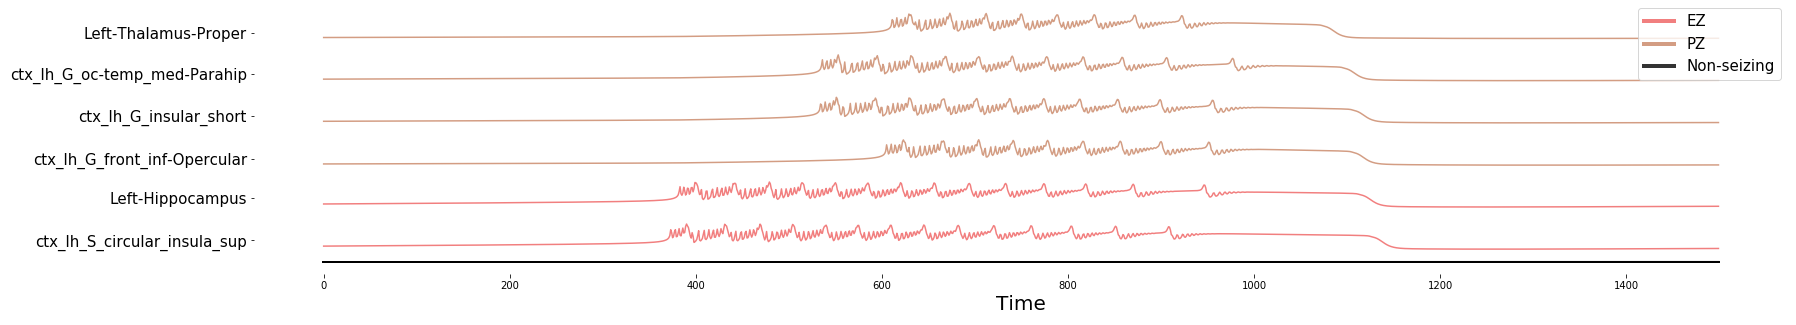
\includegraphics[width=\textwidth]{figures/source_activity_syn_data.png}
    \caption{Source activity}
  \end{subfigure}
  \begin{subfigure}{\linewidth}
    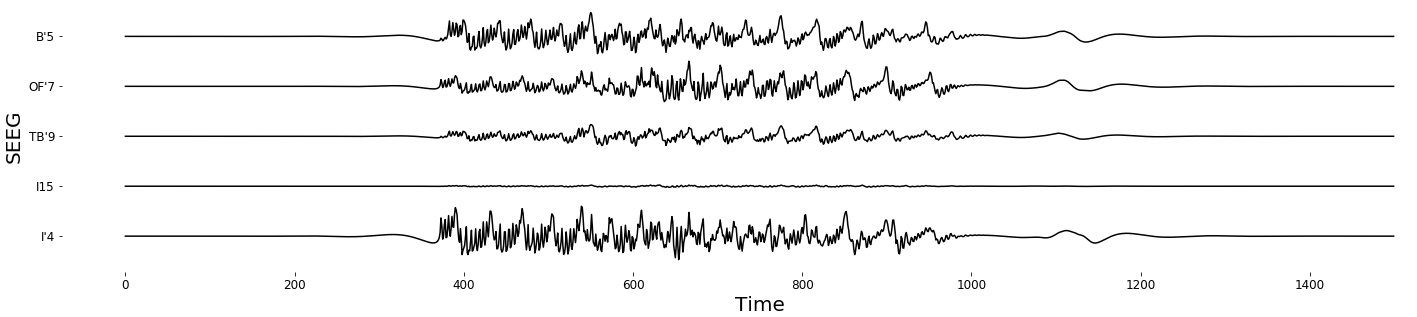
\includegraphics[width=\textwidth]{figures/seeg_syn_data.png}
    \caption{SEEG activity}
  \end{subfigure}
  \caption{Simulated seizure propagation pattern}
  \label{fig:syn-data}
\end{figure}
\subsection*{Modeled data features}
Given appropriate parameter values 2D Epileptor can capture some of the important characteristics of a seizure namely seizure onset and seizure length, which are sufficient for the purposes of identifying spatio-temporal seizure propagation patterns. Log. SEEG power encompasses both these features and hence forms a good candidate data feature that can be modeled using 2D Epileptor. See figure \ref{fig:data-features}
\begin{figure}[h!]
  \centering
  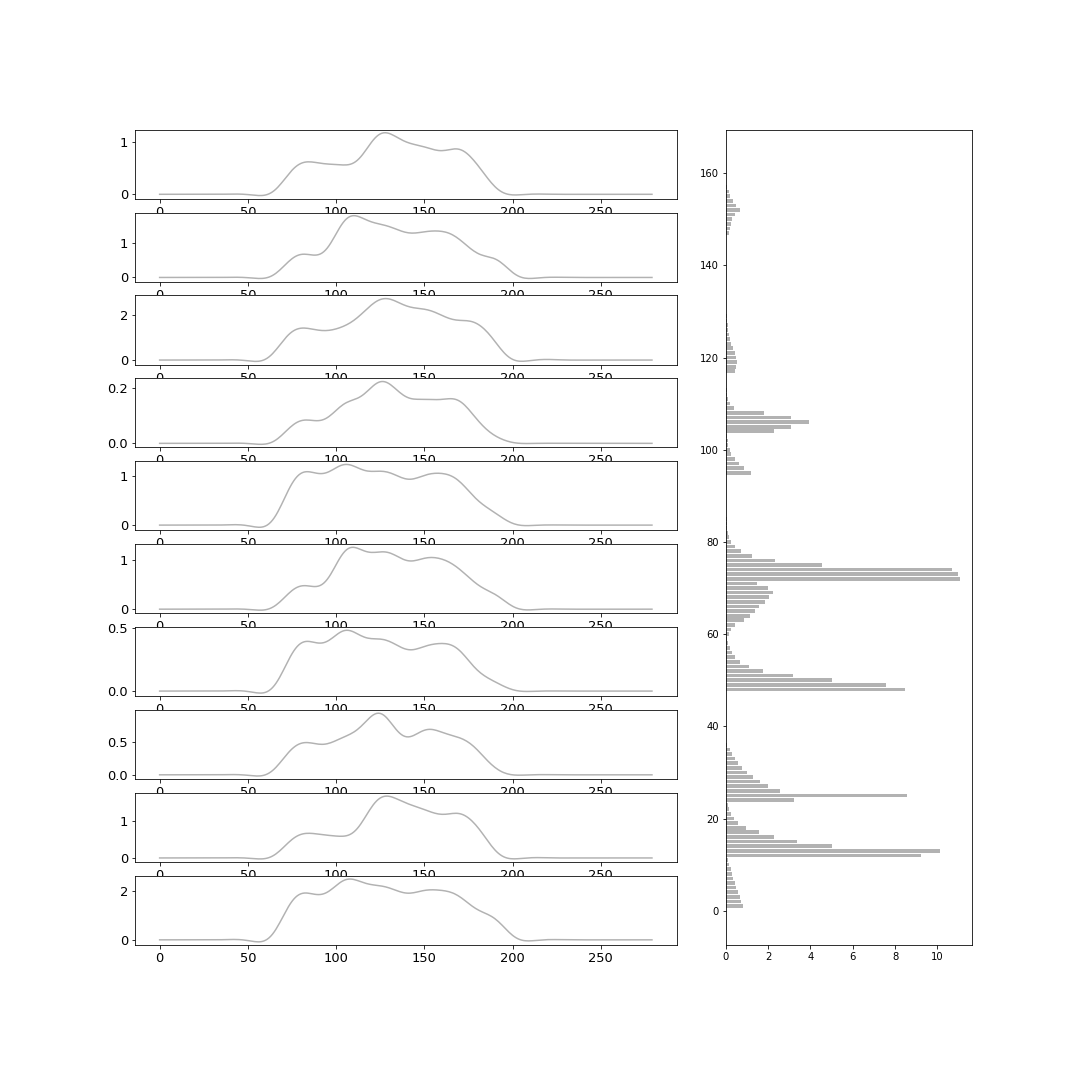
\includegraphics[width=\textwidth]{figures/modelled_data_features.png}
  \caption{Modeled data features. SEEG log power of 10 sensors(left) and total power per sensor(right)}
  \label{fig:data-features}
\end{figure}
\section*{Model}

\section*{Results}
\end{document}